\documentclass[12pt,fleqn]{article}
\usepackage{outlines}
\usepackage{amsfonts}
\usepackage{amsthm}
\theoremstyle{definition}
\newtheorem*{prop}{Proposition}
\newtheorem*{defn}{Definition}
\newtheorem*{ass}{Assumption}
\usepackage{fullpage}
\usepackage{url}
\usepackage{wrapfig}
% \renewcommand{\emph}{\textbf}
\setlength{\parskip}{0.5em}
\setlength{\parindent}{0em}

\usepackage{xcolor}
\usepackage{float}

\usepackage{tikz}
\usetikzlibrary{arrows.meta}
\usetikzlibrary{decorations.markings}

\usepackage{tikz-3dplot}

\usepackage{pgfplots}

\usepackage{colortbl}

% A few colors
%--------------------------------------------------------------
\definecolor{plum}{rgb}{0.36078, 0.20784, 0.4}
\definecolor{chameleon}{rgb}{0.30588, 0.60392, 0.023529}
\definecolor{cornflower}{rgb}{0.12549, 0.29020, 0.52941}
\definecolor{scarlet}{rgb}{0.8, 0, 0}
\definecolor{brick}{rgb}{0.64314, 0, 0}
\definecolor{sunrise}{rgb}{0.80784, 0.36078, 0}
\definecolor{lightblue}{rgb}{0.15,0.35,0.75}

\begin{document}

\section*{Lecture 21: Twins paradox}

The scenario: \begin{enumerate}
\item A and B meet
\item A and B part ways
\item Time passes (for both A and B)
\item A turns around
\item Time passes (for both A and B)
\item A and B meet again
\item Less time has passed for A than has passed for B
\end{enumerate}

\begin{figure}[H]
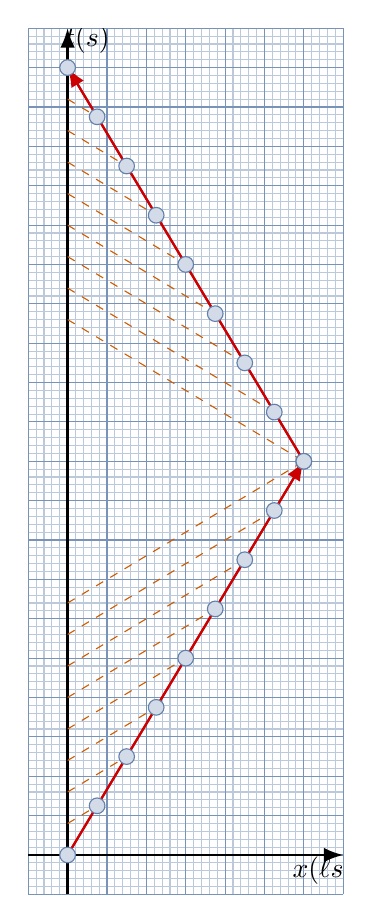
\begin{tikzpicture}[scale=0.5,domain=0:6]
	\tikzstyle{axisarrow} = [-{Latex[inset=0pt,length=7pt]}]

	% Draw the grid.
	\draw [cornflower!30,step=0.2,thin] (-1,-1) grid (7,21);
	\draw [cornflower!60,step=1.0,thin] (-1,-1) grid (7,21);

	% Clip all lines that would fall outside the grid
	\clip(-1,-1) rectangle (7,21);
	
	% Draw Axes
	\draw[thick,axisarrow] (0,-1) -- (0,21);
	\node[inner sep=0pt] at (0.5,20.7) {$t (s)$};
	\draw[thick,axisarrow] (-1,0) -- (7,0);
	\node[inner sep=0pt] at (6.5,-0.4) {$x (\ell s)$};

	
	
	\draw[scarlet,thick,axisarrow] (0,0) -- (3*10/5,10);
	\draw[scarlet,thick] plot (\x,5*\x/3);

	\draw[scarlet,thick,axisarrow] (6,10) -- (0,20);
	\draw[scarlet,thick] plot (\x,-5*\x/3+20);


	\begin{scope}
		\clip (0,0) -- (6,10) -- (0,20) -- (0,0);
    	
		\foreach \tp in {0,1,2,...,8}
		{
			\draw[dashed, sunrise] plot (\x,0.6*\x + 0.8*\tp);
		}
		
    	\foreach \tp in {0,1,2,...,8}
		{
			\draw[dashed, sunrise] plot (\x,-0.6*\x + 0.8*\tp+ 13.6);
		}
				
	\end{scope}

    	\foreach \tp in {0,1,...,8}
		{
			\node at (0.75*\tp,1.25*\tp) [circle,draw=cornflower!70,fill=cornflower!20,inner sep=2pt] {};
			}	

	    \foreach \tp in {0,1,...,8}
		{
			\node at (6-0.75*\tp,10+1.25*\tp) [circle,draw=cornflower!70,fill=cornflower!20,inner sep=2pt] {};
		}

              \end{tikzpicture} \end{figure}
              
              \newpage

\begin{outline}[enumerate]              

\1 Clarifications

\2 The last claim is a \emph{prediction} of STR

\2 According to the standard interpretation of STR, both A and B have
kept time correctly



\1 Is this a \emph{paradox}?

If a theory predicts P and not-P, then it is \emph{bad}

\1 How does STR predict this?

Some terminology:
\begin{itemize}
\item World line = path through spacetime traced by a massive object  
\item Proper time = time elapsed along a world line
\end{itemize}

The \emph{clock hypothesis} states that an ideal clock measures the
\emph{distance} along a world line

We want to define a notion of ``distance'' between points $p,q\in
M$. The best way to do this is indirectly, via talking about the
vectors at the points $p$ and $q$

\begin{ass} The space $T_p$ is isomorphic to the space $T_q$ for all
  $p,q\in M$. We use the name $V$ for this space. \end{ass}

\begin{defn} A \emph{vector space} $V$ over the real numbers
  $\mathbb{R}$ has a distinguished element $0\in V$ and two
  operations:
\begin{itemize}
\item Addition: $v,w\mapsto v+w$
\item Scalar multiplication: $a,v\mapsto av$
\end{itemize} \end{defn}

\begin{defn} An \emph{inner product} $\eta$ on $V$ is a function from
  pairs of elements of $V$ to $\mathbb{R}$ that is:
\begin{itemize}
\item Symmetric
\item Linear in both arguments
\item Semi-definite: for each $u\in V$ there is a $v\in V$ such that
  $\eta (u,v)\neq 0$.
\end{itemize} \end{defn}

\begin{defn} A \emph{subspace} $W$ of $V$ is a subset that contains
  $0$ and is closed under the addition and scalar multiplication
  operations. \end{defn}

\begin{defn} We say that $\eta$ is positive definite on $W$ just in
  case $\eta (v,v)\geq 0$ for all $v\in W$, and $\eta (v,v)=0$ only if
  $v=0$. \end{defn}

\begin{defn} The \emph{signature} of $\eta$ is a pair of non-negative
  integers $(n^+,n^-)$, where $n^+$ is the maximal possible dimension
  for a positive definite subspace, and $n^-$ is the maximal possible
  dimension for a negative definite subspace. \end{defn}

\begin{ass} Minkowski spacetime is a metric affine space with
  signature $(1,3)$, although we often represent it by an affine space
  with signature $(1,1)$. \end{ass}

\begin{defn} For $u\in V$, we let $\| u\| = |\langle u,u\rangle |^2$,
  which we consider to be the generalized length of $u$. \end{defn}

\begin{prop}[Reverse triangle inequality] Let $u,v\in V$ be timelike
  vectors. Then $\| u+v\|\geq \| u\| + \| v\|$, with equality iff
  $u=av$ for some $a\in \mathbb{R}$. \end{prop}


\1 What, if anything is the takeaway point of this example?

\2 Is there no objective notion of the amount of time between events?
Whose time is real?

``You have two hours to complete and submit the exam''


\1 Confusions

\2 The physical situations of A and B are exactly the same

\2 The difference is explained by the fact that A accelerates and B
does not

\2 The faster a clock moves the slower it ticks





\1 Clarifications for the technically interested

\2 The world lines of A and B are \emph{not} symmetric. ``$\alpha$ is
straight'' is definable in the language of STR. Since $\alpha$ is bent
and $\beta$ is straight, they are not equivalent.

\2 In fact, spacetime distance is invariant under symmetries. Hence,
it is impossible to map a worldline $\alpha$ to a longer worldline
$\beta$. (Paradox avoided: two observers will always agree about
comparisons of proper times.)

Contrast with two observers' judgments of whether $x$ occurred before
$y$, when $x$ and $y$ are spacelike related

%% Kinky trajectories are shorter than straight trajectories 

\end{outline}









\end{document}


%%% Local Variables:
%%% mode: latex
%%% TeX-master: t
%%% End:
